\begin{frame}
    \centering
    \begin{figure}[H]
        
\includegraphics[keepaspectratio, width=0.7\paperwidth, height=\paperheight]{LeeLogo}
    \end{figure}
    Informatik: Programmieren\\
    \emoji{abacus} Kapitel 03 (Teil 1): \textbf{Variablen und Parameter}
\end{frame}

% command to make sure colorboxes don't create whitespace between code lines
\fboxsep=.6pt

% default settings for listings
\lstset{style=TigerJython, basicstyle=\scriptsize\ttfamily,escapechar=!}

\begin{frame}[fragile]{Weshalb braucht es Parameter?}
\vspace{-.5cm}
\begin{columns}
\begin{column}{.4\pagewidth}
\begin{lstlisting}
from gturtle import *
makeTurtle()

def quadrat50():
	repeat 4:
		fd(50)
		rt(90)
		
def quadrat100():
	repeat 4:
		fd(100)
		rt(90)

def quadrat150():
	repeat 4:
		fd(150)
		rt(90)
		
quadrat50()
quadrat100()
quadrat150()
\end{lstlisting}
\end{column}
\begin{column}{.3\pagewidth}
\begin{figure}[H]
\centering
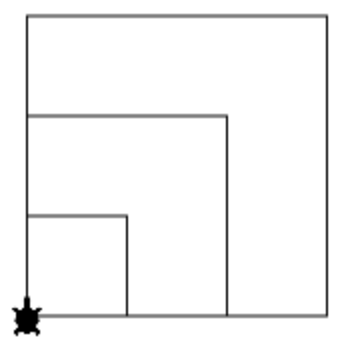
\includegraphics[width=0.7\linewidth]{GrundlagenInfo/00_Programmieren/Figures/drei-quadrate}
\end{figure}
\end{column}
\end{columns}
\vspace{.5cm}
$\rightarrow$ \textbf{Wunsch}: Ein einziger Befehl mit variabler Länge!
\end{frame}

\begin{frame}[fragile]{Ein Befehl für viele Quadrate}
\begin{columns}
\begin{column}{.4\pagewidth}
\begin{lstlisting}
from gturtle import *
makeTurtle()

def quadrat(!\only<1>{laenge}\only<2->{\colorbox{CarnationPink}{la\tikzmark{arrowTo1}enge}}!):
	repeat 4:
		fd(!\only<1-2>{laenge}\only<3->{\colorbox{CarnationPink}{la\tikzmark{arrowTo2}enge}}!) 
		rt(90)

quadrat(!\only<1>{50}\only<2->{\colorbox{CarnationPink}{5\tikzmark{arrow1From}0}}!)
quadrat(!\only<1-3>{100}\only<4->{\colorbox{CarnationPink}{1\tikzmark{arrow2From}00}}!)
quadrat(!\only<1-3>{150}\only<4->{\colorbox{CarnationPink}{1\tikzmark{arrow3From}50}}!)
\end{lstlisting}
\end{column}
\begin{tikzpicture}[overlay,remember picture]
\only<2->{
    \draw[red,-stealth] (arrow1From.north) to[bend right] node[right, xshift=.2cm, fill=RoyalBlue,text=white,rounded corners] {\emoji{handshake} Übergabe} (arrowTo1);
    }
\only<3->{
    \draw[red,-stealth] (arrowTo1.south) to[bend right] (arrowTo2);
    }
    
\only<4->{
    \draw[red,-stealth] (arrow2From.south) to[bend right] (arrowTo1);
    \draw[red,-stealth] (arrow3From.south) to[bend right] (arrowTo1);
    }
\end{tikzpicture}
\begin{column}{.3\pagewidth}
\begin{figure}[H]
\centering
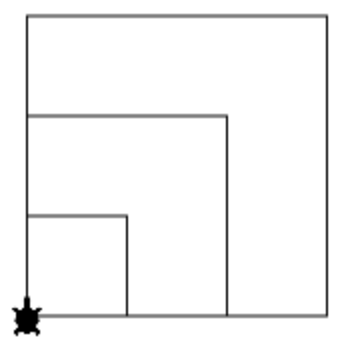
\includegraphics[width=0.7\linewidth]{GrundlagenInfo/00_Programmieren/Figures/drei-quadrate}
\end{figure}
\end{column}
\end{columns}
\end{frame}


\begin{frame}[fragile]{Mehrere Parameter}
\begin{columns}
\begin{column}{.5\textwidth}
\begin{lstlisting}
from gturtle import *
makeTurtle()

def farb_vieleck(ecken, farbe):
    spc(farbe)
    repeat ecken:
        fd(50)
        rt(360/ecken)

farb_vieleck(3,"red")
farb_vieleck(6,"green")
farb_vieleck(4,"blue")
\end{lstlisting}
\end{column}
\begin{column}{.5\textwidth}
\begin{figure}
\centering
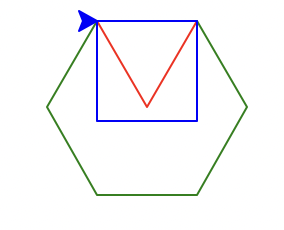
\includegraphics[width=0.3\linewidth]{GrundlagenInfo/00_Programmieren/Figures/mehrere-parameter}
\end{figure}
\end{column}
\end{columns}
\only<2->{
\vspace{.5cm}
$\rightarrow$ Man kann beliebig viele Parameter aneinanderreihen!}
\only<3->{\lstinline|def meine_funktion(p1, p2, p3, ...)|}
\end{frame}

\begin{frame}[fragile]{Variablen}
Was sind \textbf{Variablen}?
\begin{itemize}[<+->]
\item \textbf{Parameter} sind Variablen
\item Ein Wort, das einen \tib{veränderbaren} (=variablen) Wert enthält.
\item Variablenname darf (fast) frei gewählt werden
\begin{itemize}
\item Name muss mit Buchstaben beginnen (nicht: \verb|1meinname, _abc|)
\item Kein von Python reserviertes Wort (\lstinline|def, if, repeat| etc.)
\item Falls zusammengesetzter Name, immer durch \textit{underscore getrennt }\emoji{camel} \textit{camel case}, z.B.: \lstinline|meinName|
\item \textbf{Sinnvoller} und \textbf{sprechender} Name!
\end{itemize}
\end{itemize}
\end{frame}

\begin{frame}[fragile]{Auftrag}
\begin{itemize}
\item Lesen Sie den Kasten ``neue Konzepte und Begriffe'' auf S. 39
\item Lesen Sie Beispiel 3.3 und 3.4
\item \aufgabebox{Aufgaben 3.1 - 3.7}
\item \abgabebox{Aufgaben 3.2, 3.6 (Abgabe auf Moodle)}
\end{itemize}

\end{frame}